\documentclass[tikz,border=6pt]{standalone}
\usepackage{tikz}
\usepackage{amsmath,amssymb,bm}
\usetikzlibrary{shapes.geometric, shapes.arrows, arrows.meta, positioning,
                fit, backgrounds, calc, decorations.pathreplacing}

\definecolor{hbmorange}{RGB}{230,136,28}
\definecolor{l2purple}{RGB}{138,43,226}
\definecolor{smgreen}{RGB}{44,160,44}
\definecolor{regblue}{RGB}{70,130,180}
\definecolor{accentred}{RGB}{214,39,40}

\begin{document}
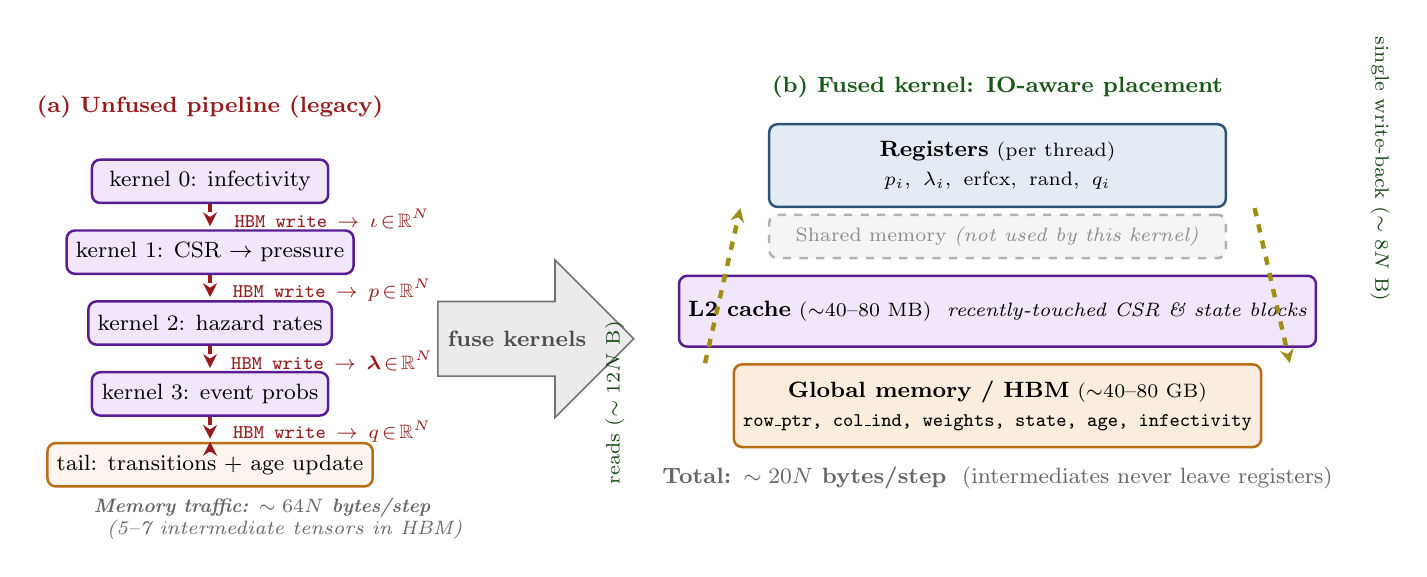
\begin{tikzpicture}[
    level/.style={rectangle, rounded corners=3pt, line width=0.9pt,
                  align=center, font=\footnotesize},
    hbm/.style={level, draw=hbmorange!80!black, fill=hbmorange!15,
                minimum width=5.8cm, minimum height=1.05cm},
    l2/.style={level, draw=l2purple!65!black, fill=l2purple!12,
               minimum width=4.6cm, minimum height=0.9cm},
    sm/.style={level, draw=smgreen!60!black, fill=smgreen!12,
               minimum width=3.4cm, minimum height=0.8cm},
    regs/.style={level, draw=regblue!65!black, fill=regblue!15,
                 minimum width=2.4cm, minimum height=0.7cm},
    datarow/.style={font=\scriptsize\ttfamily, align=left, inner sep=1pt,
                    text=black!70},
    flow/.style={-{Stealth[length=5pt,width=5pt]}, line width=0.9pt,
                 color=black!65},
    badflow/.style={flow, line width=1.2pt, color=accentred!70!black,
                    dashed},
    goodflow/.style={flow, line width=1.2pt, color=smgreen!45!orange},
    annot/.style={font=\scriptsize\itshape, text=black!60},
    sectitle/.style={font=\footnotesize\bfseries},
]

%======================================================================
% LEFT PANEL: unfused pipeline -- materialize 5-7 O(N) tensors to HBM
% between kernels.
%======================================================================
\node[sectitle, text=accentred!70!black]
     at (0.0, 4.85) {(a) Unfused pipeline (legacy)};

% 4 small kernel launches, each writing a full O(N) intermediate to HBM.
\foreach \lab [count=\k from 0] in
   {infectivity, CSR $\to$ pressure, hazard rates, event probs} {
    \node[l2, minimum width=3.0cm, minimum height=0.55cm]
         (kern\k) at (0.0, 3.9 - \k*0.90) {kernel \k: \lab};
}
\node[hbm, minimum width=3.0cm, minimum height=0.55cm, fill=hbmorange!8]
     (endkern) at (0.0, 3.9 - 4*0.90) {tail: transitions + age update};

% HBM dump between each kernel: labels showing what is materialized.
\foreach \lab [count=\k from 0] in
   {$\iota\!\in\!\mathbb{R}^{N}$, $p\!\in\!\mathbb{R}^{N}$,
    $\bm{\lambda}\!\in\!\mathbb{R}^{N}$, $q\!\in\!\mathbb{R}^{N}$} {
    \draw[badflow]
         ($(kern\k.south) + (0,0)$) -- ($(kern\k.south) + (0,-0.28)$);
    \node[datarow, text=accentred!70!black]
         at ($(kern\k.south) + (1.55, -0.19)$)
         {\texttt{HBM write $\to$ \lab}};
}
\draw[badflow]
     ($(kern3.south)+(0,-0.45)$) -- ($(endkern.north)+(0,0)$);

% Summary numbers underneath
\node[annot, align=left, anchor=north west]
     at (-1.6, 0)
     {\textbf{Memory traffic: $\sim 64N$ bytes/step}\\
      \;\;(5--7 intermediate tensors in HBM)};

%======================================================================
% MIDDLE: arrow indicating "fusion" transformation
%======================================================================
\begin{scope}[shift={(3.9, 1.9)}]
    \node[single arrow, draw=black!55, line width=0.6pt,
          fill=black!8, minimum width=2.0cm, minimum height=0.9cm,
          font=\footnotesize\bfseries, text=black!70]
         {fuse kernels};
\end{scope}


%======================================================================
% RIGHT PANEL: memory-hierarchy pyramid (fused kernel placement).
% Labels live inside each level; a single upward read arrow on the
% left exterior and a single downward write-back on the right exterior
% hug the pyramid, so no arrow ever crosses a box.
%======================================================================
\begin{scope}[shift={(10.0, 0)}]
    \node[sectitle, text=smgreen!55!black]
         at (0.0, 5.1) {(b) Fused kernel: IO-aware placement};

    \def\boxw{5.8cm}

    % Stack: fastest on top, slowest on bottom -- all equal width.
    \node[regs, minimum width=\boxw, minimum height=1.05cm, align=center]
         (lreg) at (0, 4.1)
         {\textbf{Registers} {\scriptsize(per thread)}\\[1pt]
          {\scriptsize\itshape $p_i,\ \lambda_i,\ \mathrm{erfcx},\ \mathrm{rand},\ q_i$}};

    \node[level, draw=black!30, dashed, fill=black!4,
          minimum width=\boxw, minimum height=0.55cm, align=center,
          text=black!45, font=\scriptsize]
         (lsm) at (0, 3.20)
         {Shared memory \textit{(not used by this kernel)}};

    \node[l2, minimum width=\boxw, minimum height=0.9cm, align=center]
         (lL2) at (0, 2.25)
         {\textbf{L2 cache} {\scriptsize($\sim$40--80~MB)}\ \
          {\scriptsize\itshape recently-touched CSR \& state blocks}};

    \node[hbm, minimum width=\boxw, minimum height=1.05cm, align=center]
         (lhbm) at (0, 1.05)
         {\textbf{Global memory / HBM} {\scriptsize($\sim$40--80~GB)}\\[1pt]
          {\scriptsize\ttfamily row\_ptr, col\_ind, weights, state, age, infectivity}};

    % Read path: one straight vertical arrow on the LEFT exterior,
    % label placed FURTHER out so its rotated bounding box sits fully
    % outside the stack (previous layout clipped the rotated text into
    % the L2 box; anchor=east positions the right edge of the pre-
    % rotation text at the anchor point, so after a 90-degree ccw
    % rotation the text extends leftward from the anchor).
    \draw[goodflow, line width=1.6pt, dashed, >={Stealth[scale=2]}]
         ([xshift=-0.35cm]lhbm.north west) --
         ([xshift=-0.35cm]lreg.south west);
    \node[annot, text=smgreen!45!black, rotate=90,
          anchor=east, font=\scriptsize]
         at ([xshift=-0.80cm]lL2.west) {reads ($\sim 12N$ B)};

    % Write-back: one straight vertical arrow on the RIGHT exterior
    \draw[goodflow, line width=1.6pt, dashed, >={Stealth[scale=2]}]
         ([xshift=0.35cm]lreg.south east) --
         ([xshift=0.35cm]lhbm.north east);
    \node[annot, text=smgreen!45!black, rotate=-90,
          anchor=east, font=\scriptsize]
         at ([xshift=0.80cm]lL2.east) {single write-back ($\sim 8N$ B)};

    \node[annot, align=center, anchor=north, font=\footnotesize]
         at (0, 0.40)
         {\textbf{Total: $\sim 20N$ bytes/step}\ \
          (intermediates never leave registers)};
\end{scope}

\end{tikzpicture}
\end{document}
